% ======================================================================
% Beamer deck for the in-silico microwave-reheat study (group talk).
% Build:  pdflatex mw_reheat_slides.tex   (twice; figures from
%         make_figs.py + make_slide_figs.py)
% Internal draft — program data-rights review before wider circulation.
% All numbers trace to the recorded run artifacts (see the paper draft
% mw_reheat_draft.tex and REBUILD CHANGELOG [0.1.20]-[0.1.31]).
% ======================================================================
\documentclass[aspectratio=169,10pt]{beamer}
\usetheme[progressbar=frametitle]{metropolis}
\metroset{numbering=fraction,block=fill}
\usepackage{booktabs}

\definecolor{krfviolet}{HTML}{5B2D8F}
\definecolor{okgreen}{HTML}{1E7A46}
\definecolor{badred}{HTML}{A93A2C}
\setbeamercolor{progress bar}{fg=krfviolet}
\setbeamercolor{alerted text}{fg=krfviolet}
\setbeamercolor{title separator}{fg=krfviolet}

\newcommand{\good}[1]{\textcolor{okgreen}{#1}}
\newcommand{\bad}[1]{\textcolor{badred}{#1}}

\title{Microwave reheating of e-beam-pumped excimer plasmas}
\subtitle{observable, real, and marginal --- an in-silico study across
three independent models}
\author{Cooper K.\ Watson}
\institute{Texas A\&M University \\[1ex]
{\tiny Internal draft --- program data-rights review before wider
circulation. All numbers regenerate from recorded run artifacts.}}
\date{August 28, 2026}

\begin{document}

\maketitle

% ----------------------------------------------------------------------
\begin{frame}{The question, and how it was asked}
\textbf{Hybrid pumping:} keep the e-beam as primary ionizer, add
microwave power (during the pulse or in the afterglow) to reheat the
electrons and harvest more excimer formation. Does it help?
\vspace{1ex}
\begin{itemize}
  \item \alert{Twin pairs}: identical runs $\pm$ a prescribed-power
        microwave window. Marginal $m=\Delta E_L/E_{\rm MW}$; blended
        $\Delta\eta$ with the microwave joules in the denominator;
        fluorescence $E_{\rm fl}$ = the experimental observable.
  \item \alert{Three independent electron treatments}: 26-species 0-D
        engine on LoKI-MC swarm tables; the same engine on
        PIC/MCC-measured rates; an independently written 1-D
        discharge-pumped fluid model (two-term Boltzmann).
  \item \alert{Decidability ladder}: a sign counts only if it survives
        numerics $\to$ rate-tier swap $\to$ $\times\frac13..\times3$
        rate brackets $\to$ the independent model. Otherwise it is
        reported \emph{undecided}, with the measurement that decides it.
\end{itemize}
\end{frame}

% ----------------------------------------------------------------------
\begin{frame}{The answer in three lines}
\begin{enumerate}
  \item \good{\textbf{Reheating is a robust observable.}} The
        gain-proportional fluorescence rises in \textbf{8/8}
        benchmarks, on both rate tiers, and in the independent model
        ($+1.5\%$ to $+12\%$).
  \item \good{\textbf{One laser-positive channel is real}} --- afterglow
        reheat of a high-margin, still-extracting cavity:
        ${\sim}+10\%$ per microwave joule, surviving \textbf{41/41}
        rate brackets, tier swap (sibling cell), 1-D replication, and
        a \textbf{16.5$\sigma$} placebo-calibrated artifact test.
  \item \bad{\textbf{Exploiting it is very difficult.}} No benchmark
        moves its blended efficiency by more than
        \textbf{0.006 percentage points} at program-representative
        coupling; five quantitative walls stand between ``real'' and
        ``useful.''
\end{enumerate}
\end{frame}

% ----------------------------------------------------------------------
\begin{frame}{1. The observable: fluorescence responds everywhere --- efficiency does not}
\begin{center}
\small
\begin{tabular}{lcccc}
\toprule
case & $\eta_0$ & afterglow $m$ & $\Delta\eta$ (pp) & $\Delta E_{\rm fl}$ \\
\midrule
high-power cell, 2 atm & 1.54\% & $-2.8\%$ & $-0.0055$ & $+0.48$ mJ \\
X-band chamber column  & 2.16\% & $-10.4\%$ & $-0.0036$ & $+2.15$ mJ \\
Ar-optimized           & 4.95\% & $-2.1\%$ & $-0.0056$ & $+5.12$ mJ \\
\alert{Ne-optimized}   & 6.19\% & \good{$+10.0\%$} & \good{$+0.0024$} & $+1.30$ mJ \\
KrF anchor (1985)      & 0.70\% & $-0.0\%$ & $-0.0003$ & $+0.47$ mJ \\
ArF anchor, 1.09 atm   & 6.13\% & $-1.3\%$ & $-0.0031$ & $+14.8$ mJ \\
\bottomrule
\end{tabular}
\end{center}
\vspace{1ex}
\alert{The trap for experiment design:} the diagnostic
(fluorescence $\propto$ gain) rises \emph{even where laser output
falls} --- six of eight afterglow cases. A fluorescence increase is
not an efficiency statement.
\end{frame}

% ----------------------------------------------------------------------
\begin{frame}{2. The real channel: late extraction, not afterglow harvest}
\begin{columns}[T]
\begin{column}{0.46\textwidth}
\vspace{1ex}
\begin{itemize}
  \item Every direct excimer-formation row is heavy-particle; heating
        the electrons cuts \emph{both} supply lines
        (F$^-$ $\times0.13$, precursor$^*$ $\times0.37$).
  \item The one positive case gains by \alert{late extraction}: the
        high-margin cavity is still draining while the window runs
        ($\Delta E_L \gg \Delta E_{\rm fl}$).
  \item Sign survives \textbf{all 41} rate-bracket / literature
        variants ($+8.3\%$ to $+12.9\%$) $\to$
  \item Cross-framework witnesses: kinetic tier $+9.5\%$ (sibling
        cell); 1-D model $+10.1\%$ at its finest timestep.
\end{itemize}
\end{column}
\begin{column}{0.52\textwidth}
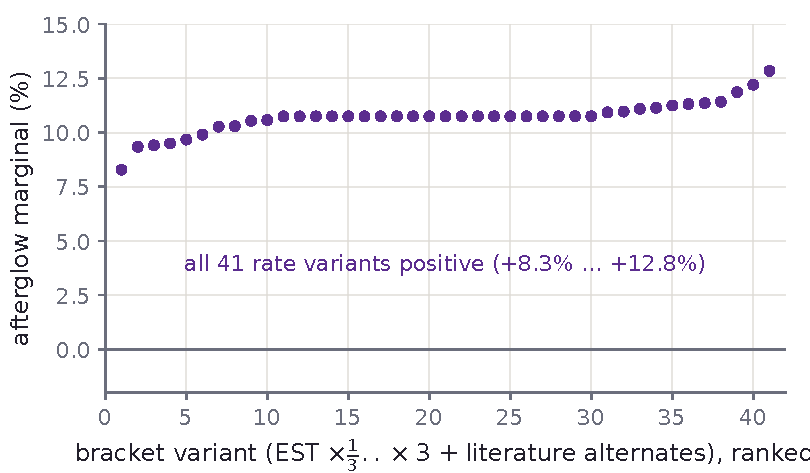
\includegraphics[width=\textwidth]{s_bracket.pdf}
\end{column}
\end{columns}
\end{frame}

% ----------------------------------------------------------------------
\begin{frame}{2. Verified in 1-D: the mechanism's own fingerprints}
\begin{columns}[T]
\begin{column}{0.5\textwidth}
\centering
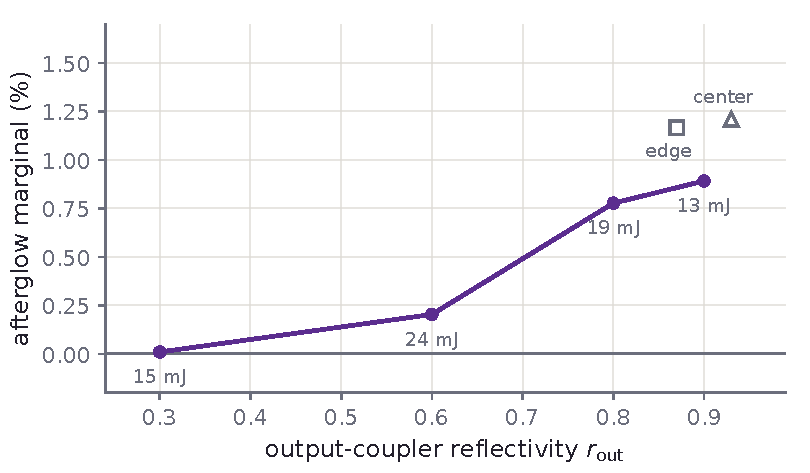
\includegraphics[width=\textwidth]{s_margin.pdf}
\end{column}
\begin{column}{0.5\textwidth}
\centering
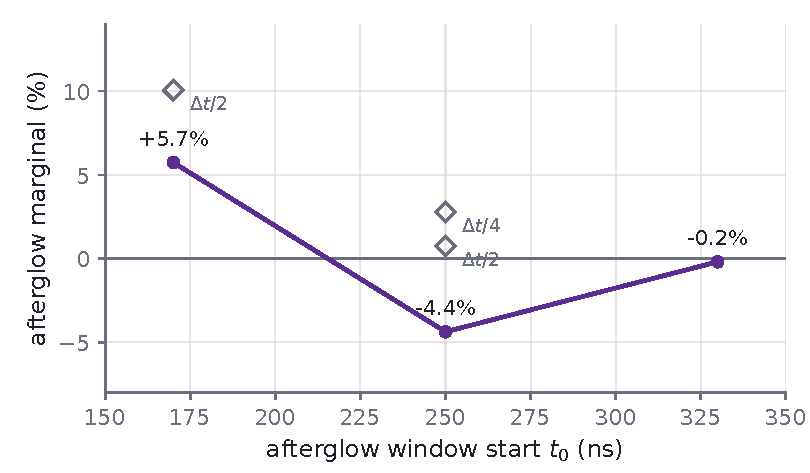
\includegraphics[width=\textwidth]{s_timing.pdf}
\end{column}
\end{columns}
\vspace{0.5ex}
\begin{itemize}
  \item \textbf{Margin (left):} marginal rises monotonically with
        $r_{\rm out}$ while the \emph{absolute} output peaks at 0.6
        --- it tracks photon lifetime, not laser performance.
        Edge/center/uniform deposition: \alert{where} is second-order.
  \item \textbf{Timing (right):} $+5.7\%\to+10.1\%$ under $\Delta t$
        refinement at full drain overlap; decays to ${\approx}0$ past
        the drain (the $-4.4\%$ dip was a $\Delta t$ artifact ---
        caught by refinement). \alert{When} is first-order.
\end{itemize}
\end{frame}

% ----------------------------------------------------------------------
\begin{frame}{2. Not a numerical artifact: a placebo-calibrated $16.5\sigma$}
\begin{itemize}
  \item Per solver setting (7: tolerance decades, atol, step cap, and
        the \emph{independent Radau integrator}), the twin runs three
        ways: off / 500 kW signal / \alert{1 W placebo} --- the
        placebo twin difference calibrates the numerical differencing
        noise \emph{in situ}.
  \item Exact Student-$t$ discovery: $p_0 = 1.7\times10^{-61}$
        (13 dof) $\Rightarrow$ \alert{$Z = 16.5\sigma$}; $2\times10^5$
        null toys: zero exceedances; 95\% CL$_{\rm s}$ band
        $[8.5980, 8.5982]$ mJ excludes zero by $1.4\times10^5$ s.e.
  \item Worst single bracket variant alone: $z \approx 4\times10^4$;
        the noise would need to be wrong by $\times4\times10^4$ to
        drop to $3\sigma$. Conservative by construction (the placebo
        carries real small-signal physics). Self-testing machinery +
        negative control.
  \item 1-D: differencing floor measured by a power ladder
        ($8\times10^{-4}$ mJ) --- the signal sits $\times300$ above it.
\end{itemize}
\vspace{0.5ex}
{\small\emph{Scope:} rejects a numerics-noise origin. Shared
model error is covered separately: two unrelated codebases agree,
energy ledger closes to $10^{-13}$, 197-test suite, bracket program.}
\end{frame}

% ----------------------------------------------------------------------
\begin{frame}{3. Why it is very difficult: five walls}
\begin{columns}[T]
\begin{column}{0.5\textwidth}
\vspace{0.5ex}
\small
\begin{enumerate}
  \item \textbf{The ceiling:} $|\Delta\eta| \le 0.006$ pp everywhere
        --- the marginal must beat the cell's own $\eta$ to pay.
  \item \textbf{Conductivity pinning:} the afterglow settles at
        ${\lesssim}2$ Td at \emph{any} power (to 1 GW); the useful
        channel needs 20--30 Td.
  \item \textbf{Supply-chain inversion:} heating cuts both excimer
        feedstocks (KrF and ArF).
  \item \textbf{Wall-plug (right):} frequency-blind below 0.3 THz;
        only magnetrons $\times$ the fragile $+12\%$ clear the bar
        (= the program-stated ${\sim}7\%$ current e-beam wall-plug).
        The 2-mm skin makes uniform coupling an upper bound.
  \item \textbf{The during-pulse sign:} one uncertain rate wide
        (next slide).
\end{enumerate}
\end{column}
\begin{column}{0.48\textwidth}
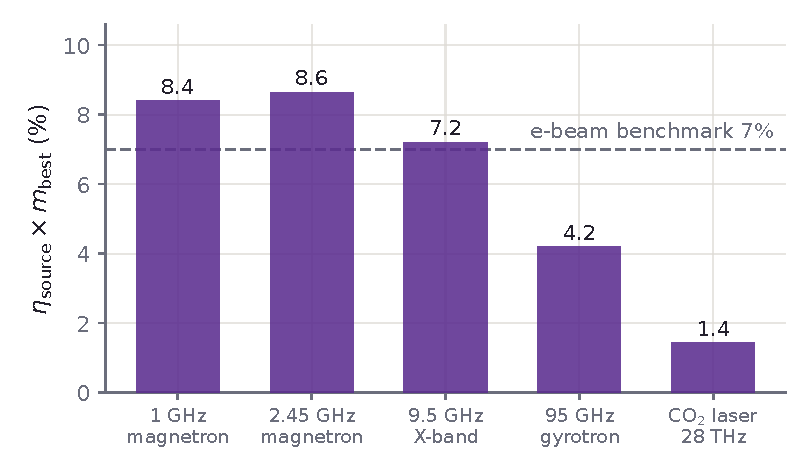
\includegraphics[width=\textwidth]{s_wallplug.pdf}
\end{column}
\end{columns}
\end{frame}

% ----------------------------------------------------------------------
\begin{frame}{3. The during-pulse sign: one rate wide, and $\Delta t$-fragile}
\begin{columns}[T]
\begin{column}{0.5\textwidth}
\centering
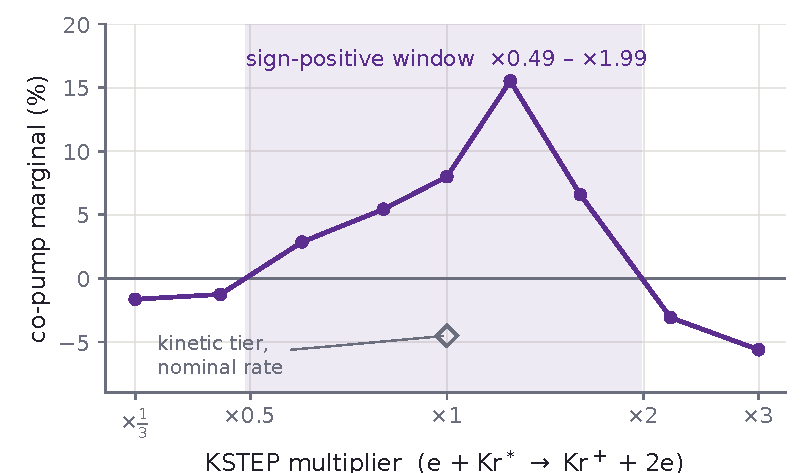
\includegraphics[width=\textwidth]{s_kstep.pdf}
\end{column}
\begin{column}{0.5\textwidth}
\centering
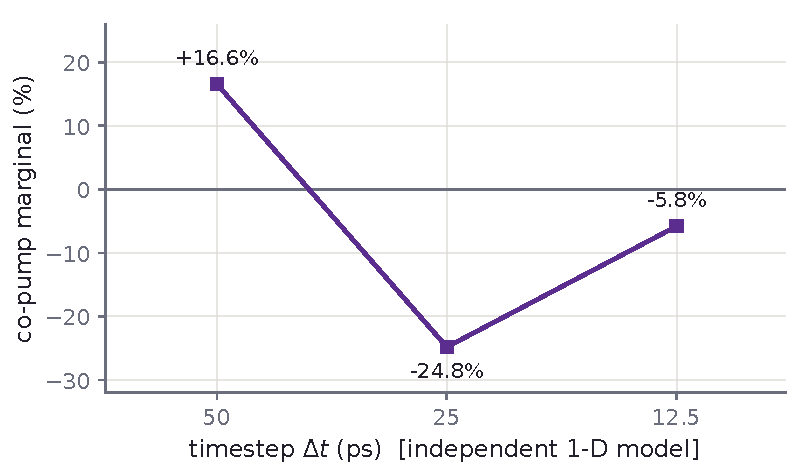
\includegraphics[width=\textwidth]{s_dtseries.pdf}
\end{column}
\end{columns}
\vspace{0.5ex}
\begin{itemize}
  \item \textbf{Left (0-D):} co-pump sign positive \emph{iff} KSTEP
        ($e+\mathrm{Kr}^*\!\to\mathrm{Kr}^++2e$) lies within
        $\times0.49$--$\times1.99$ of nominal; current knowledge
        ($\times3$) straddles both crossings $\Rightarrow$
        \alert{undecidable today, decided by a factor-2 rate
        determination}.
  \item \textbf{Right (1-D):} the coarse-$\Delta t$ $+16.6\%$ dies
        under refinement --- small-or-negative at fine steps.
\end{itemize}
\end{frame}

% ----------------------------------------------------------------------
\begin{frame}{What to do with this}
\begin{itemize}
  \item \textbf{Measure one rate}: Kr$^*$ stepwise ionization to a
        factor of 2 (literature adjudication / driven PIC sampling /
        experiment) decides the co-pump sign.
  \item \textbf{Run the twin-shot experiment} in a high-margin cell:
        window on/off at fixed fill; scanning the window delay traces
        the drain curve --- the mechanism's direct signature. Shot
        counts follow from measured twin variances.
  \item \textbf{Close the denominator}: quoting any measured marginal
        needs the \emph{absorbed} microwave energy --- a full-wave
        deposition map (the 2-mm skin vs the cell), not forward power.
  \item \textbf{Perspective}: the levers that actually move
        efficiency remain conventional --- F$_2$ fraction, pressure,
        optics, buffer: a measured ladder $1.54\%\to6.19\%$, roughly
        $10^3\times$ any electromagnetic effect found here.
\end{itemize}
\end{frame}

% ----------------------------------------------------------------------
\begin{frame}{Summary}
\begin{enumerate}
  \item Reheating \good{works as an observable}: fluorescence responds
        in every configuration, in every model. The diagnostic will
        see the microwave --- do not mistake it for efficiency.
  \item The afterglow gain in a still-extracting cavity is
        \good{real}: ${\sim}+10\%$ per microwave joule, bracket-proof
        (41/41), 1-D-verified ladder by ladder, and
        $16.5\sigma$ against the numerics-artifact null.
  \item Converting it to device efficiency is \bad{very difficult}:
        $\le 0.006$ pp at feasible coupling, five quantified walls,
        and the one larger channel hangs on a single rate known to
        $\times3$.
\end{enumerate}
\vspace{1ex}
\centering
\alert{One rate to measure, one regime to test, one observable not to
be fooled by.}
\end{frame}

% ----------------------------------------------------------------------
\appendix
\begin{frame}{Backup: the full benchmark sweep (swarm tier, corrected engine)}
\begin{center}
\footnotesize
\begin{tabular}{lccccc}
\toprule
 & & \multicolumn{2}{c}{afterglow} & \multicolumn{2}{c}{co-pump} \\
case & $\eta_0$ & $m$ & $\Delta\eta$ (pp) & $m$ & $\Delta\eta$ (pp) \\
\midrule
program class, 3 atm (Ar) & no lasing & --- & --- & --- & --- \\
program class, 3 atm (Ne) & no lasing & --- & --- & --- & --- \\
high-power cell, 2 atm & 1.54\% & $-2.8\%$ & $-0.0055$ & $+12.5\%$ & $+0.0029$ \\
X-band chamber column & 2.16\% & $-10.4\%$ & $-0.0036$ & $-1.9\%$ & $-0.0004$ \\
Ar-optimized & 4.95\% & $-2.1\%$ & $-0.0056$ & $+1.3\%$ & $-0.0010$ \\
Ne-optimized & 6.19\% & $+10.0\%$ & $+0.0024$ & $+5.1\%$ & $-0.0002$ \\
KrF anchor (1985) & 0.70\% & $-0.0\%$ & $-0.0003$ & $+3.0\%$ & $+0.0002$ \\
ArF anchor, 1.09 atm & 6.13\% & $-1.3\%$ & $-0.0031$ & $+5.7\%$ & $-0.0001$ \\
\bottomrule
\end{tabular}
\end{center}
\vspace{0.5ex}
{\small Kinetic tier (5/8): re-running on the independently derived
PIC-measured rate set flips the \emph{signs} of these few-percent
marginals (HYPER co-pump $+12.5\to-2.7\%$; Ar-opt afterglow
$-2.1\to+9.5\%$) while the $\le0.006$-pp magnitude ceiling holds on
both sets (max kinetic $|\Delta\eta|$ 0.0036 pp). ``Sign not
tier-stable'' means exactly that --- the answer's sign depends on
which rate set you believe, not that a bug is suspected. Full record:
\texttt{mw\_reheat\_draft.pdf} + REBUILD CHANGELOG [0.1.20]--[0.1.33].}
\end{frame}

% ----------------------------------------------------------------------
\begin{frame}{Backup: the arithmetic of a blended gain, derated}
\textbf{With and without, exactly (Ne-optimized cell):} without
microwave $\eta_0 = 7.773\,\mathrm{J}/125.49\,\mathrm{J} =
\alert{6.194\%}$; with the afterglow window $\eta =
7.781\,\mathrm{J}/125.57\,\mathrm{J} = \alert{6.197\%}$.
To first order (exact to the digits shown):
\[
  \Delta\eta \;\simeq\; (\eta_c\, m - \eta_0)\,
  \frac{E_{\rm RF}}{E_{\rm tot}},
  \qquad m = +10.0\%/\text{absorbed J},\;\; \eta_c = \text{absorbed
  fraction.}
\]
\vspace{-1.5ex}
\begin{columns}[T]
\begin{column}{0.55\textwidth}
\small
\begin{itemize}
  \item Intrinsic gain needs $\eta_c > \eta_0/m = \alert{62\%}$
        absorbed.
  \item Wall-plug gain needs $\eta_{\rm src}\eta_c\, m > 7\%$: a 72\%
        magnetron needs $\eta_c \ge 97\%$; X-band and gyrotron need
        $>100\%$ --- \bad{excluded at any realistic coupling} (at an
        8\% bar, excluded outright).
  \item Fresnel reflection off the collisional plasma face
        ($\nu \approx 2\times10^{12}$ s$^{-1}$), at
        $n_e = 10^{19}/10^{20}/10^{21}$ m$^{-3}$:
        2.45 GHz: 5/42/76\%; \; 9.5 GHz: 0/17/58\%; \;
        \alert{95 GHz: 0/0/20\%}.
\end{itemize}
\end{column}
\begin{column}{0.43\textwidth}
\small
\textbf{Demonstration point} (intrinsic accounting):
Ne-opt cell ($\eta_0$ 6.2\%, margin ${\sim}19$), afterglow window
beam-off$+10$ ns $\times$ 150 ns, \alert{95 GHz} launch
($\eta_c \approx 0.75$--$0.9$ plausible; the low source efficiency is
irrelevant to intrinsic bookkeeping).
\smallskip

Expected: $\Delta\eta \approx +0.001$ to $+0.04$ pp for
$E_{\rm RF} = 0.1$--$2$ J --- an mJ-class, $16.5\sigma$-measurable
$\Delta E_L$, \emph{not} a device lever.
\end{column}
\end{columns}
\end{frame}

\end{document}
